% ============================================================================
\section{Introduction}
\label{sec:intro}
% ============================================================================
\PARstart{I}{ndonesian} employers compute and withhold Income Tax Article 21 (PPh 21) from the pay of each employee every month, so an error in the tax rules reaches every payslip of the company. These rules change often: 13 regulatory events changed the PPh 21 computation for permanent employees between 2023 and 2026, and seven of them were issued in 2025 (Fig.~\ref{fig:timeline}). Government Regulation (PP) 58/2023 and Minister of Finance Regulation (PMK) 168/2023 replaced the annualized monthly method with average effective rates (TER) from January 2024. Both were issued in the last week of December 2023~\cite{pp58_2023,pmk168_2023}. Five of the 13 events took effect retroactively. One of them is PMK 10/2025, which introduced government-borne tax (DTP) for employees in labor-intensive sectors. Because PMK 10/2025 was issued on 4 February 2025 but covers January 2025, a January payroll that was correct when it ran owed a correction a month later~\cite{pmk10_2025}.

\begin{figure*}[!t]
\centering
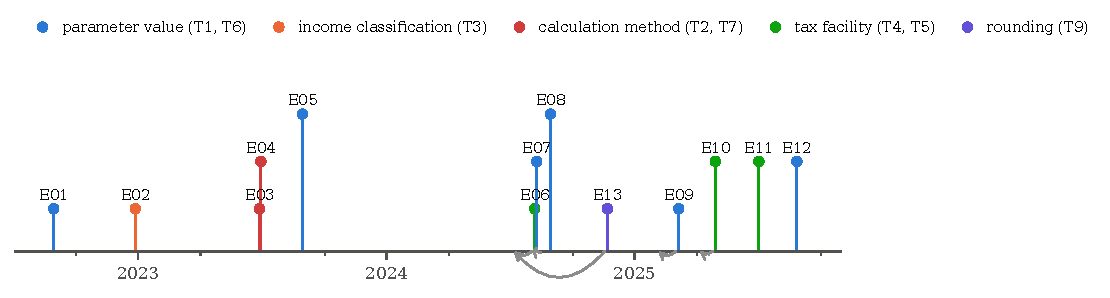
\includegraphics[width=\textwidth]{figs/fig_timeline.pdf}
\caption{Regulatory events that changed PPh 21 for permanent employees in 2023--2026, placed at their issue dates.}
\label{fig:timeline}
\end{figure*}

The government regulation is only one layer of the rules that a payslip follows. Each company adds its own pay policies on allowances, overtime, the religious holiday allowance (THR), and employer-borne tax through a collective labor agreement or company regulation. The same regulation therefore changes the payslips of two companies differently. A regulatory change can also silently alter the effect of a company clause.

Because payroll software usually encodes both layers in program code or spreadsheets~\cite{ramadhani2021grossup,kusuma2026pph21}, every change needs new code. The commit histories of two open-source PPh 21 calculators show that TER was added 26 and 915 days after PP 58/2023 was issued. A knowledge-based system (KBS) separates the rules from the code that executes them~\cite{merigoux2021catala}, but the work moves to keeping the knowledge base (KB) current. Large language models (LLMs) can turn legal text into structured rules~\cite{janatian2023texttostructure} although they are unreliable when asked to compute tax directly~\cite{nay2024taxattorneys,dahl2024legalfictions}.

Prior work leaves three gaps for a payroll system that must follow such a stream of changes.
\begin{enumerate}
  \item \emph{No LLM-assisted tax KB is maintained through a sequence of real changes.} Work that combines LLMs with tax rules formalizes the law at one point in time~\cite{veeramani2026neurosymbolic,lorenzo2025translating,jurayj2026tax}. The closest work updates a tax program by one legal year with LLM-written candidates and a majority vote~\cite{goganikhiabani2025maintaining}, without a chain of updates and without testing earlier periods.
  \item \emph{No executable tax KB handles retroactive rules together with company policies.} Versioned legal knowledge graphs record how the text of a norm evolves~\cite{demartim2025satgraph}, but their rules are not executed. Payroll and tax systems do not separate company policies from the regulation they build on~\cite{dumancic2021payroll,alhawari2026payroll}.
  \item \emph{No evaluation measures the payslips that result from LLM-drafted updates.} Existing studies score each drafted rule or answer on its own~\cite{goganikhiabani2025maintaining,jurayj2026tax}, not the payslips of a company that receives the updates one after another.
\end{enumerate}

This study addresses the three gaps with an adaptive KBS for PPh 21 (Fig.~\ref{fig:architecture}). The novelty of the system is an executable two-layer knowledge graph that LLM-drafted updates keep current and that records the legal validity of every rule and the date on which the rule became known. Deterministic gates check each drafted update before a behavioral consensus proposes it or abstains. A company therefore receives retroactive government regulations and changes of its own policies without any change of program code. A deterministic engine computes the tax. A software engineer who maintains the company's human capital (HC) systems such as payroll approves each proposal. The contributions of this study are as follows:
\begin{itemize}
  \item \emph{A two-layer bitemporal knowledge base with LLM-assisted updates.} Government regulations and company policies are separate layers of one RDF knowledge graph with executable rules. Their bitemporal records let the engine recalculate months already paid when a retroactive rule arrives while the earlier results stay reproducible. An update pipeline drafts each change three times from the document, checks every draft with six deterministic gates, and proposes an update only when the drafts agree.
  \item \emph{A chained, payslip-level evaluation on real document streams.} Five real companies with one installation each received the regulations of 2023--2026, their labor agreements, and distractor documents in the order of issue. Every payslip was scored against a reference knowledge base checked by a tax practitioner and compared with a code-based update made 26 days after each issue.
  \item \emph{Evidence on payslip accuracy and manual work.} Payslip accuracy on the payroll date exceeded that of the code-based update in four of the five companies when an HC software engineer approved the proposals. A completeness gate added after the evaluation brought the fifth company to the level of the code-based update in a replay of the recorded drafts. The engineer wrote updates by hand for 11 of the 138 documents.
\end{itemize}

Section~\ref{sec:background} summarizes PPh 21 and its changes, and Section~\ref{sec:related} reviews related work. Section~\ref{sec:system} describes the system and Section~\ref{sec:design} the evaluation, whose results are presented in Section~\ref{sec:results} and discussed in Section~\ref{sec:discussion} before Section~\ref{sec:conclusion} concludes the paper.
